\chapter{Experimental Results}

%Replace \lipsum with text.
% You may have as many sections as you please. This is just for reference.

\section{Transfer of Data from RTDS to server}
\begin{figure}
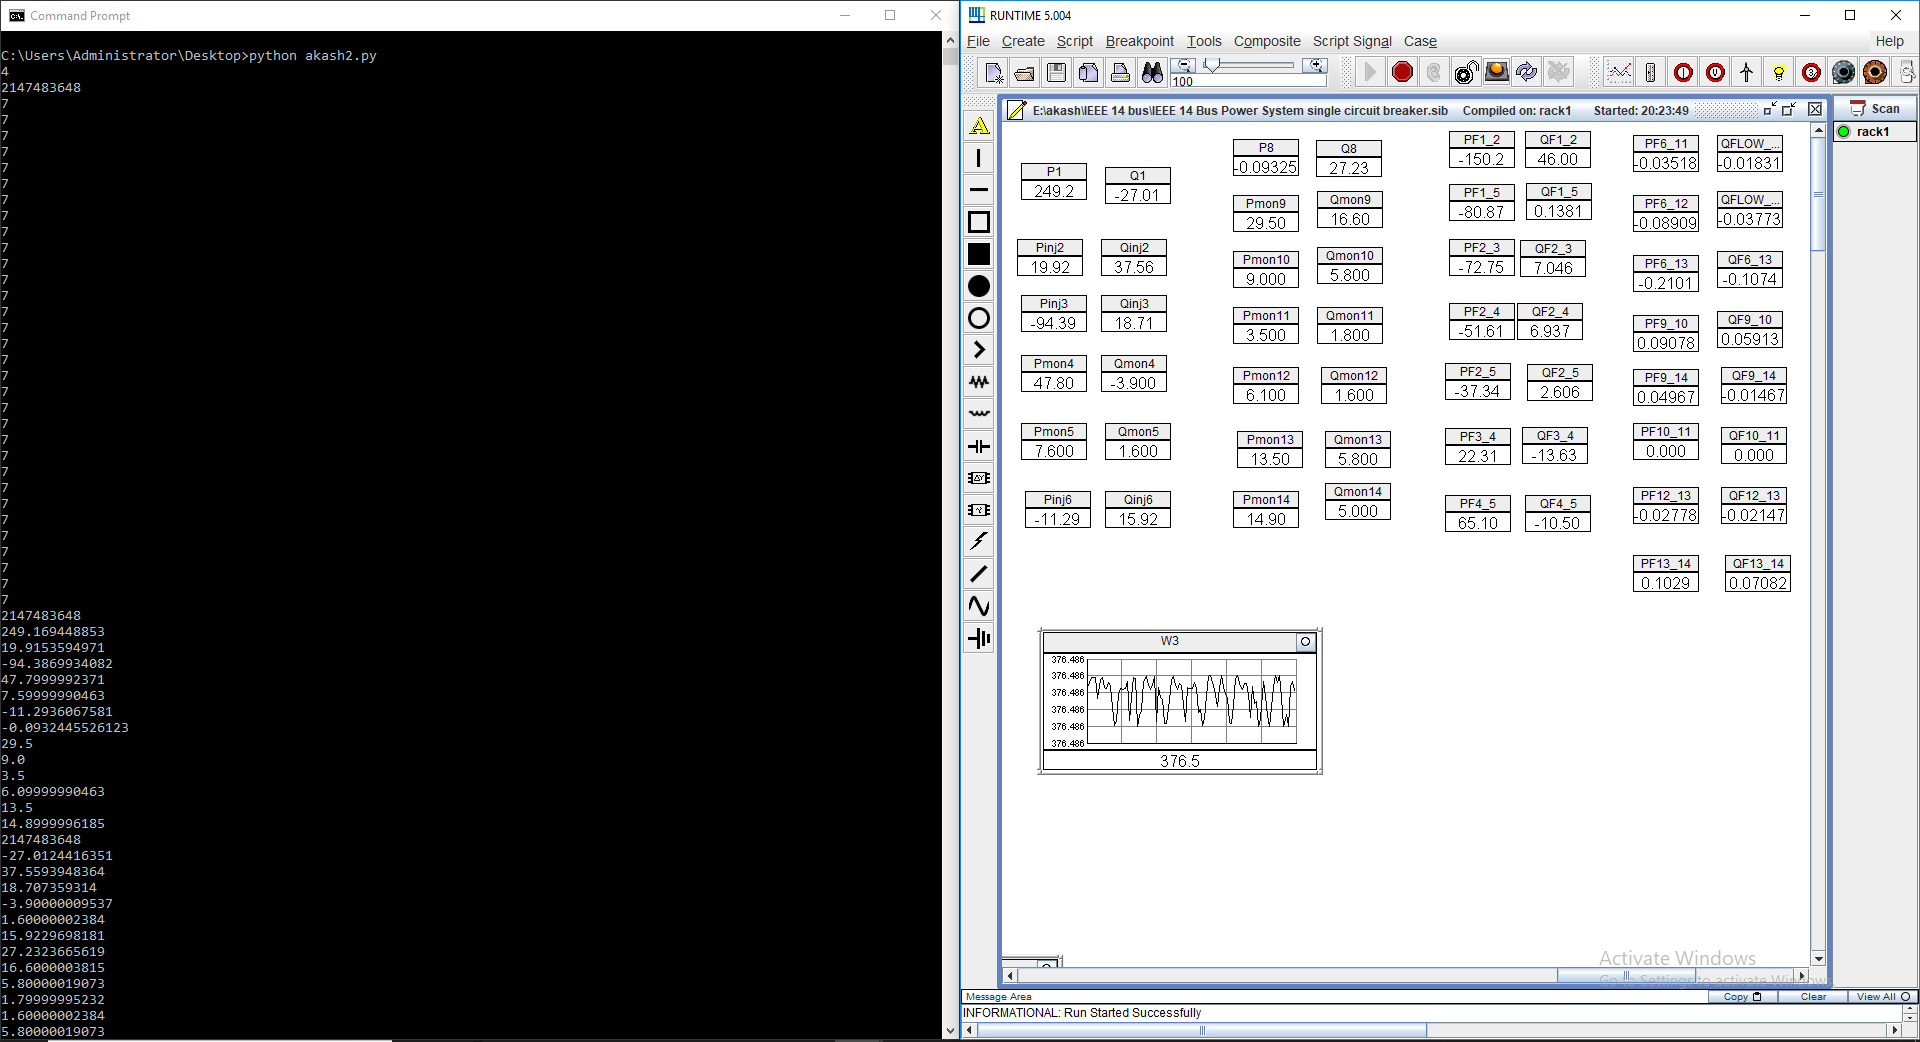
\includegraphics[width=\textwidth]{Figures/response_dt_cb.png}
\caption{Transfer of real and reactive power injections and flows from RTDS (right) to server (left), Observing circuit breaker status}
\label{fig:data_transfer_cb_status}
\end{figure}

\begin{figure}
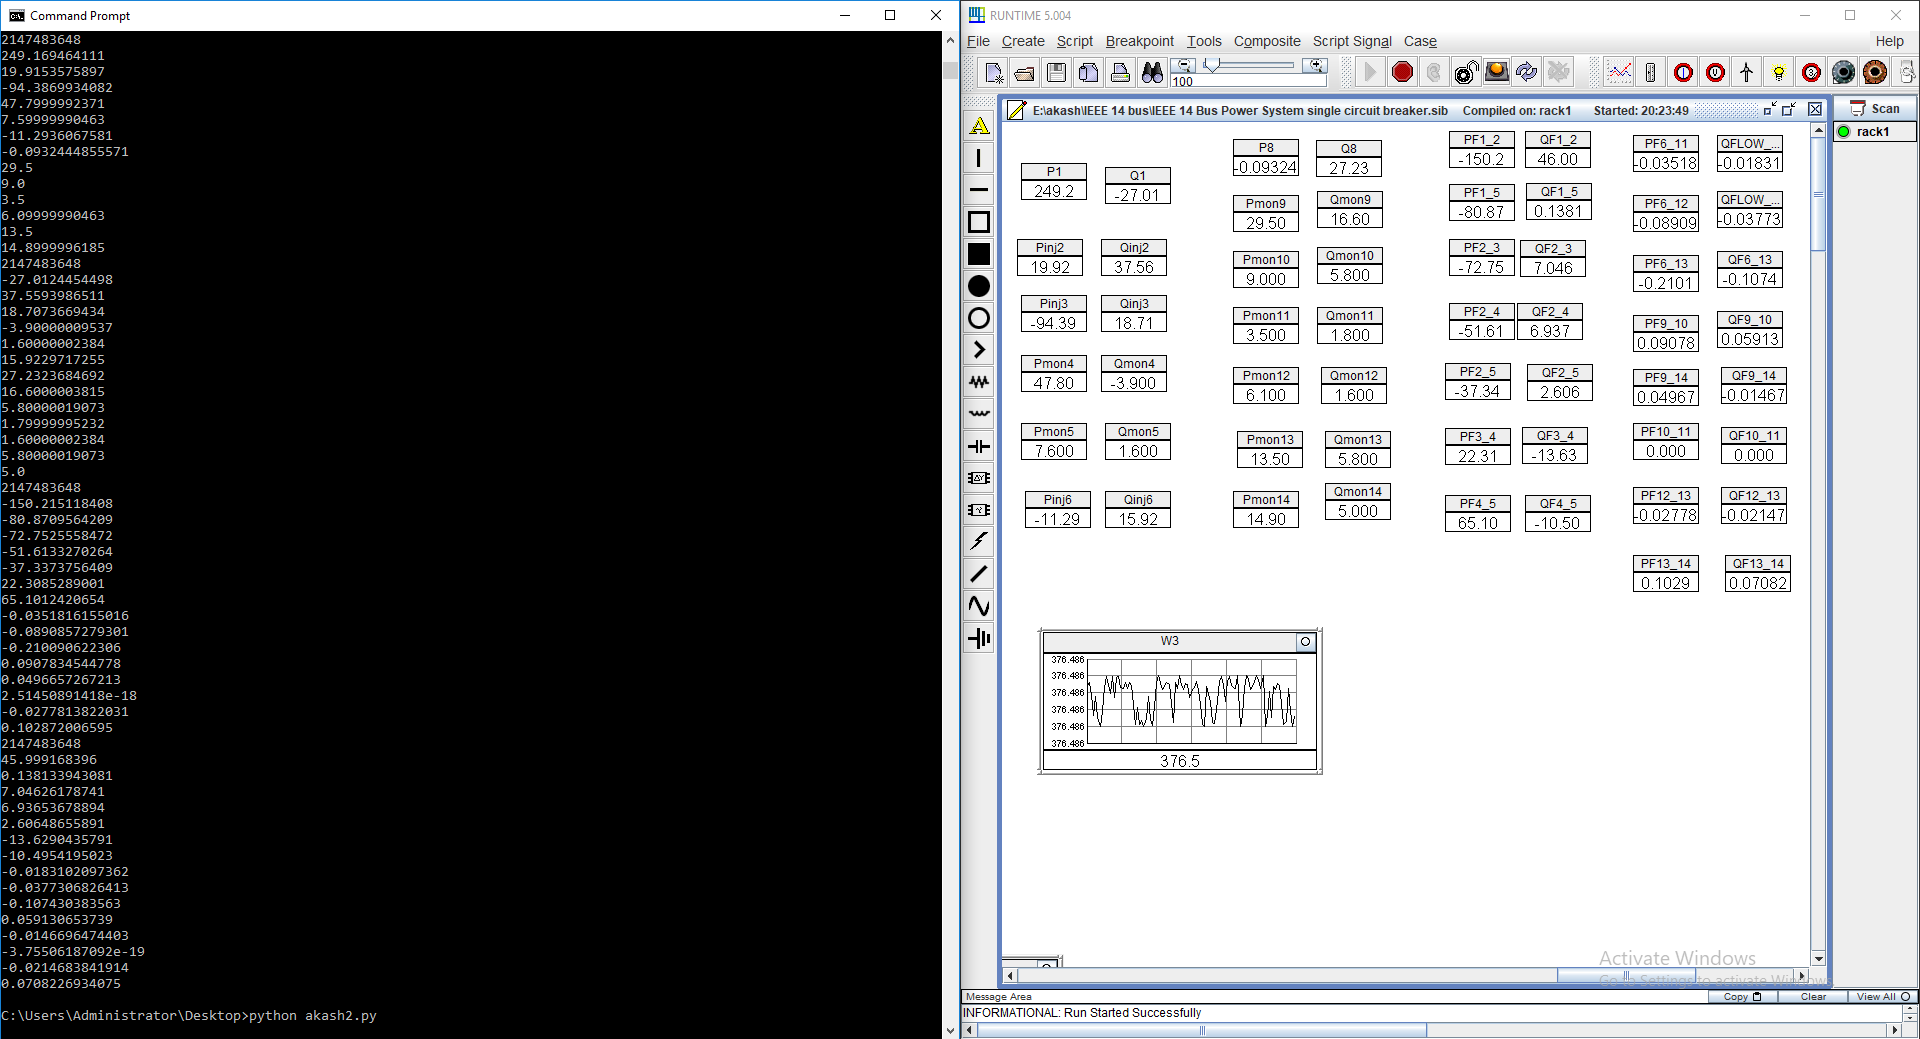
\includegraphics[width=\textwidth]{result_dt2.png}
\caption{Transfer of real and reactive power injections and flows from RTDS (right) to server (left)}
\label{fig:data_transfer}
\end{figure}

In Figure ~\ref{fig:data_transfer}, we observe real time data transfer from RTDS via GTNET-SKT to our server, which we built using a python script running on the Desktop. Here the measurements come in the order described in chapter 3 (Real injection then reactive . The value 2147483648 ($2^{32}-1$) is the status number for the set of measurements. All bits are 1, signifying all measurements are available. In Figure ~\ref{fig:data_transfer_cb_status}, we observe the availability status of all circuit breakers in the system. The first number is the case\_number, and 4 represents 14 bus system. Circuit breakers status number is also 2147483648, signifying all circuit breakers are available. Circuit breaker measurement of 7 represents all 3 phases are ON (3 bits are 1).\\
The graph is the frequency response curve of the system, in rad/s. The system operates at $376.5/2 \pi=60Hz$ with very little fluctuation.\\

This shows that we have been able to extract all the available measurements, and identify which measurement belongs to which variable, without using many extra measurement variables.

\section{Observability Analysis}


\section{State Estimation}
